\documentclass[10pt]{article}
\usepackage{tikz}
\usetikzlibrary{shapes.misc}
\usepackage[margin=0cm]{geometry}
\pagestyle{empty}
\tikzstyle{every node}=[cross out, draw, red]

\begin{document}

\vspace*{\fill}
\begin{center}
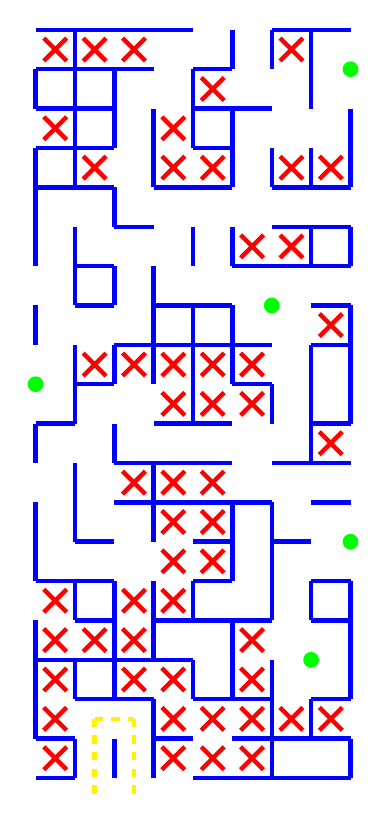
\begin{tikzpicture}[x=0.5cm, y=-0.5cm, ultra thick, blue]
% Walls
    \draw (0,0) -- (4,0);
    \draw (6,0) -- (8,0);
    \draw (0,1) -- (3,1);
    \draw (4,1) -- (5,1);
    \draw (0,2) -- (2,2);
    \draw (4,2) -- (6,2);
    \draw (0,3) -- (2,3);
    \draw (4,3) -- (5,3);
    \draw (0,4) -- (2,4);
    \draw (3,4) -- (5,4);
    \draw (6,4) -- (8,4);
    \draw (2,5) -- (3,5);
    \draw (6,5) -- (8,5);
    \draw (1,6) -- (2,6);
    \draw (5,6) -- (8,6);
    \draw (1,7) -- (2,7);
    \draw (3,7) -- (5,7);
    \draw (7,7) -- (8,7);
    \draw (2,8) -- (6,8);
    \draw (7,8) -- (8,8);
    \draw (1,9) -- (2,9);
    \draw (5,9) -- (6,9);
    \draw (0,10) -- (1,10);
    \draw (3,10) -- (5,10);
    \draw (7,10) -- (8,10);
    \draw (2,11) -- (5,11);
    \draw (6,11) -- (8,11);
    \draw (2,12) -- (6,12);
    \draw (7,12) -- (8,12);
    \draw (1,13) -- (2,13);
    \draw (4,13) -- (5,13);
    \draw (6,13) -- (7,13);
    \draw (0,14) -- (2,14);
    \draw (4,14) -- (5,14);
    \draw (7,14) -- (8,14);
    \draw (1,15) -- (2,15);
    \draw (3,15) -- (6,15);
    \draw (7,15) -- (8,15);
    \draw (0,16) -- (4,16);
    \draw (1,17) -- (3,17);
    \draw (4,17) -- (6,17);
    \draw (7,17) -- (8,17);
    \draw (0,18) -- (1,18);
    \draw (3,18) -- (4,18);
    \draw (5,18) -- (8,18);
    \draw (0,19) -- (1,19);
    \draw (4,19) -- (8,19);
    \draw (0,1) -- (0,2);
    \draw (0,3) -- (0,6);
    \draw (0,7) -- (0,8);
    \draw (0,10) -- (0,11);
    \draw (0,12) -- (0,14);
    \draw (0,15) -- (0,18);
    \draw (1,0) -- (1,4);
    \draw (1,5) -- (1,7);
    \draw (1,8) -- (1,10);
    \draw (1,11) -- (1,13);
    \draw (1,14) -- (1,15);
    \draw (1,16) -- (1,17);
    \draw (1,18) -- (1,19);
    \draw (2,1) -- (2,3);
    \draw (2,4) -- (2,5);
    \draw (2,6) -- (2,7);
    \draw (2,8) -- (2,9);
    \draw (2,10) -- (2,11);
    \draw (2,14) -- (2,17);
    \draw (2,18) -- (2,19);
    \draw (3,2) -- (3,4);
    \draw (3,6) -- (3,9);
    \draw (3,11) -- (3,13);
    \draw (3,14) -- (3,16);
    \draw (3,17) -- (3,19);
    \draw (4,1) -- (4,3);
    \draw (4,5) -- (4,6);
    \draw (4,7) -- (4,10);
    \draw (4,14) -- (4,15);
    \draw (4,16) -- (4,17);
    \draw (5,0) -- (5,1);
    \draw (5,2) -- (5,4);
    \draw (5,5) -- (5,6);
    \draw (5,7) -- (5,9);
    \draw (5,12) -- (5,14);
    \draw (5,15) -- (5,17);
    \draw (6,0) -- (6,1);
    \draw (6,3) -- (6,4);
    \draw (6,9) -- (6,10);
    \draw (6,12) -- (6,15);
    \draw (6,16) -- (6,19);
    \draw (7,0) -- (7,2);
    \draw (7,3) -- (7,4);
    \draw (7,5) -- (7,6);
    \draw (7,8) -- (7,11);
    \draw (7,14) -- (7,15);
    \draw (7,17) -- (7,18);
    \draw (8,2) -- (8,4);
    \draw (8,5) -- (8,6);
    \draw (8,7) -- (8,10);
    \draw (8,14) -- (8,17);
    \draw (8,18) -- (8,19);
% Pillars
    \fill[green] (8,1) circle(0.2);
    \fill[green] (6,7) circle(0.2);
    \fill[green] (0,9) circle(0.2);
    \fill[green] (8,13) circle(0.2);
    \fill[green] (7,16) circle(0.2);
% Inner points in accessible cul-de-sacs
    \node at (0.5,0.5) {};
    \node at (1.5,0.5) {};
    \node at (2.5,0.5) {};
    \node at (6.5,0.5) {};
    \node at (4.5,1.5) {};
    \node at (0.5,2.5) {};
    \node at (3.5,2.5) {};
    \node at (1.5,3.5) {};
    \node at (3.5,3.5) {};
    \node at (4.5,3.5) {};
    \node at (6.5,3.5) {};
    \node at (7.5,3.5) {};
    \node at (5.5,5.5) {};
    \node at (6.5,5.5) {};
    \node at (7.5,7.5) {};
    \node at (1.5,8.5) {};
    \node at (2.5,8.5) {};
    \node at (3.5,8.5) {};
    \node at (4.5,8.5) {};
    \node at (5.5,8.5) {};
    \node at (3.5,9.5) {};
    \node at (4.5,9.5) {};
    \node at (5.5,9.5) {};
    \node at (7.5,10.5) {};
    \node at (2.5,11.5) {};
    \node at (3.5,11.5) {};
    \node at (4.5,11.5) {};
    \node at (3.5,12.5) {};
    \node at (4.5,12.5) {};
    \node at (3.5,13.5) {};
    \node at (4.5,13.5) {};
    \node at (0.5,14.5) {};
    \node at (2.5,14.5) {};
    \node at (3.5,14.5) {};
    \node at (0.5,15.5) {};
    \node at (1.5,15.5) {};
    \node at (2.5,15.5) {};
    \node at (5.5,15.5) {};
    \node at (0.5,16.5) {};
    \node at (2.5,16.5) {};
    \node at (3.5,16.5) {};
    \node at (5.5,16.5) {};
    \node at (0.5,17.5) {};
    \node at (3.5,17.5) {};
    \node at (4.5,17.5) {};
    \node at (5.5,17.5) {};
    \node at (6.5,17.5) {};
    \node at (7.5,17.5) {};
    \node at (0.5,18.5) {};
    \node at (3.5,18.5) {};
    \node at (4.5,18.5) {};
    \node at (5.5,18.5) {};
% Entry-exit paths without intersections
    \draw[dashed, yellow] (1.5,17.5) -- (2.5,17.5);
    \draw[dashed, yellow] (1.5,17.5) -- (1.5,19.5);
    \draw[dashed, yellow] (2.5,17.5) -- (2.5,19.5);
\end{tikzpicture}
\end{center}
\vspace*{\fill}

\end{document}
